\documentclass[fleqn, a4paper, 11pt, oneside]{amsart}
%\usepackage[top = 2cm, bottom = 1cm, left = 1cm, right = 1cm]{geometry}
\usepackage{exsheets, tasks}
\usepackage{amsmath, amssymb, amsthm} %standard AMS packages
\usepackage{marginnote} %marginnotes
\usepackage{gensymb} %miscellaneous symbols
\usepackage{commath} %differential symbols
\usepackage{xcolor} %colours
\usepackage{cancel} %cancelling terms
\usepackage[free-standing-units, space-before-unit]{siunitx} %formatting units
\usepackage{tikz, pgfplots} %diagrams
\usetikzlibrary{calc, hobby, patterns, intersections, decorations.markings}
\usepackage{graphicx} %inserting graphics
\usepackage{hyperref} %hyperlinks
\usepackage{datetime} %date and time
\usepackage{ulem} %underline for \emph{}
\usepackage{xfrac} %inline fractions
\usepackage{enumerate,enumitem} %numbered lists
\usepackage{float} %inserting floats
\usepackage{circuitikz}[american voltages, american currents] %circuit diagrams

\newcommand\numberthis{\addtocounter{equation}{1}\tag{\theequation}} %adds numbers to specific equations in non-numbered list of equations

\newcommand{\AxisRotator}[1][rotate=0]{
	\tikz [x=0.25cm,y=0.60cm,line width=.2ex,-stealth,#1] \draw (0,0) arc (-150:150:1 and 1);%
} %rotation symbols on axes

\theoremstyle{definition}
\newtheorem{example}{Example}
\newtheorem{definition}{Definition}

\theoremstyle{theorem}
\newtheorem{theorem}{Theorem}

\newcommand{\curl}{\mathrm{curl\,}}

\makeatletter
\@addtoreset{section}{part} %resets section numbers in new part
\makeatother

\renewcommand{\thesubsection}{(\arabic{subsection})}
\renewcommand{\thesection}{(\arabic{section})}

%section headings on left
\makeatletter
\def\specialsection{\@startsection{section}{1}%
	\z@{\linespacing\@plus\linespacing}{.5\linespacing}%
	%  {\normalfont\centering}}% DELETED
	{\normalfont}}% NEW
\def\section{\@startsection{section}{1}%
	\z@{.7\linespacing\@plus\linespacing}{.5\linespacing}%
	%  {\normalfont\scshape\centering}}% DELETED
	{\normalfont\scshape}}% NEW
\makeatother

%forces newline after subsection
\makeatletter
\def\subsection{\@startsection{subsection}{3}%
	\z@{.5\linespacing\@plus.7\linespacing}{.1\linespacing}%
	{\normalfont\itshape}}
\makeatother

\settasks{counter-format = tsk[1].}

\SetupExSheets{solution/print = true}

%opening
\title{Introduction to Linear Systems : Assignment 2}
\author
{
	Aakash Jog\\
	ID : 989323563
}
\date{\formatdate{29}{10}{2015}}

\begin{document}

\tikzset{->-/.style={decoration={
  markings,
  mark=at position #1 with {\arrow{>}}},postaction={decorate}}}

\maketitle
%\setlength{\mathindent}{0pt}

\begin{question}
	\begin{enumerate}
		\item
			The transfer function of a system is
			\begin{align*}
				G(s) & = \frac{1}{(s + 2) (s + 5)}
			\end{align*}
			Find the output, i.e. the particular solution for the input
			\begin{align*}
				u(t) & = \cos(3 t) \delta_{-1}(t)
			\end{align*}
		\item
			Consider the signal
			\begin{align*}
				p(t) & = \left( 3 + 2 e^{-t} - e^{-2 t} \right) \delta_{-1}(t)
			\end{align*}
			\begin{enumerate}
				\item
					Suppose it represents the impulse response of a system.
					Is the system stable?
				\item
					Suppose it does not represent the response of a system to a step input, with zero initial conditions, is the system stable?
			\end{enumerate}
	\end{enumerate}
\end{question}

\begin{solution}
	\begin{enumerate}
		\item
			\begin{align*}
				u(t)            & = \cos(3 t) \delta_{-1}(t) \\
				\therefore U(s) & = \frac{s}{s^2 + 9}
			\end{align*}
			Therefore,
			\begin{align*}
				Y_p(s) & = G(s) U(s) \\
                                       & = \frac{1}{(s + 1) (s + 5)} \frac{s}{s^2 + 9}
			\end{align*}
			Let
			\begin{align*}
				Y_p(s) & = \frac{A}{s + 2} + \frac{B}{s + 5} + \frac{C s + D}{s^2 + 9}
			\end{align*}
			Therefore,
			\begin{align*}
				A & = \lim\limits_{s \to -2} \frac{1}{s + 5} \frac{s}{s^2 + 9} \\
                                  & = -\frac{2}{39}                                            \\
				B & = \lim\limits_{s \to -5} \frac{1}{s + 2} \frac{s}{s^2 + 9} \\
                                  & = \frac{5}{102}
			\end{align*}
			Therefore,
			\begin{align*}
				Y_p(s)       & = \frac{-\frac{2}{39} (s^2 + 9) (s + 5) + \frac{5}{102} (s^2 + 9) (s + 2) + (C s + D) (s + 2) (s + 5)}{(s + 2) (s + 5) (s^2 + 9)} \\
				\therefore s & = \quad -\frac{2}{39} \left( s^3 + 5 s^2 + 9 s + 45 \right)                                                                       \\
                                             & \quad + \frac{5}{102} \left( s^3 + 2 s^2 + 9 s + 18 \right)                                                                       \\
                                             & \quad + (C s + D) \left( s^2 + 7 s + 10 \right)
			\end{align*}
			Therefore, solving,
			\begin{align*}
				C & = \frac{1}{442} \\
				D & = \frac{63}{442}
			\end{align*}
			Therefore,
			\begin{align*}
				Y_p(s) & = -\frac{2}{39} \frac{1}{s + 2} + \frac{5}{102} \frac{1}{s + 5} + \frac{21}{442} \frac{3}{s^2 + 9} + \frac{1}{442} \frac{s}{s^2 + 9}
			\end{align*}
			Therefore,
			\begin{align*}
				y_p(t) & = \left( -\frac{2}{39} e^{-2 t} + \frac{5}{102} e^{-5 t} + \frac{21}{442} \sin(3 t) + \frac{1}{442} \cos(3 t) \right) \delta_{-1}(t)
			\end{align*}
		\item
			\begin{enumerate}
				\item
					As $p(t)$ is the impulse response of a system, the system is stable if and only is all roots of $P(s) = G(s) = 0$ are in the left half-plane of the complex plane.
					\begin{align*}
						p(t)            & = \left( 3 + 2 e^{-t} - e^{-2 t} \right) \delta_{-1}(t) \\
						\therefore P(s) & = \frac{3}{s} + \frac{2}{s + 1} - \frac{1}{s + 2}       \\
                                                                & = \frac{4 s^2 + 12 s + 6}{s (s + 1) (s + 2)}
					\end{align*}
					Therefore, as $P(s) = 0$ has a root at $s = 0$, which is not in the left half-plane, the system is not stable.
				\item
					If $p(t)$ does not represent the step response of a system, nothing can be said about the system, as the information is not sufficient.
			\end{enumerate}
	\end{enumerate}
\end{solution}

\begin{question}
	Consider the system in the following illustration.
	\begin{figure}[H]
		\centering
		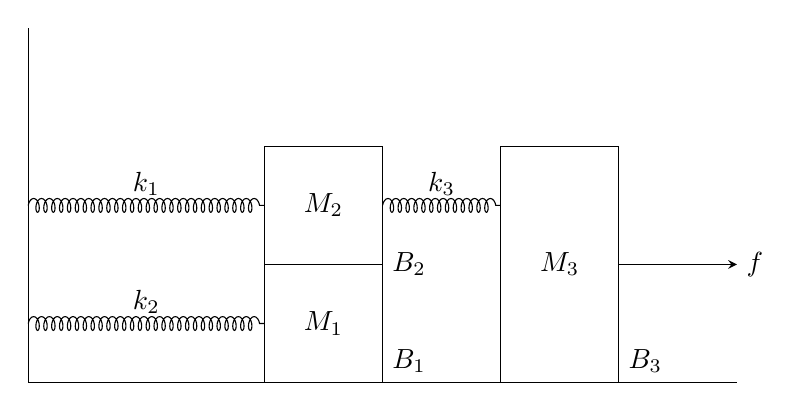
\begin{tikzpicture}[scale = 1.5]
			\def\xMIN{0};
			\def\xMAX{6};
			\def\yMIN{0};
			\def\yMAX{3};

			\def\h{1};
			\def\l{1};
			\def\F{1};

			\begin{scope}
				\draw (\xMIN,0) -- (\xMAX,0);
				\draw (0,\yMIN) -- (0,\yMAX);
			\end{scope}

			\begin{scope}
				\draw (2*\l,0) rectangle ++(\l,\h);
				\node at (2.5*\l,0.5*\h) {$M_1$};

				\draw (2*\l,\h) rectangle ++(\l,\h);
				\node at (2.5*\l,1.5*\h) {$M_2$};

				\draw (4*\l,0) rectangle ++(\l,2*\h);
				\node at (4.5*\l,\h) {$M_3$};
			\end{scope}

			\begin{scope}
				\draw [decorate, decoration = {coil, segment length = 0.1cm}] (0,0.5*\h) -- ++(2*\l,0) node [midway, above] {$k_2$};
				\draw [decorate, decoration = {coil, segment length = 0.1cm}] (0,1.5*\h) -- ++(2*\l,0) node [midway, above] {$k_1$};
				\draw [decorate, decoration = {coil, segment length = 0.1cm}] (3*\l,1.5*\h) -- ++(\l,0) node [midway, above] {$k_3$};
			\end{scope}

			\begin{scope}
				\node [above right] at (3*\l,0) {$B_1$};
				\node [right] at (3*\l,\h) {$B_2$};
				\node [above right] at (5*\l,0) {$B_3$};
			\end{scope}

			\begin{scope}[-stealth]
				\draw (5*\l,\h) -- ++(\F,0) node [right] {$f$};
			\end{scope}
		\end{tikzpicture}
	\end{figure}
	$k_i$ represent springs, $B_i$ represent viscous friction, and $M_i$ represent masses.
	The positive direction is defined to the right.
	\begin{enumerate}
		\item
			Draw an equivalent electrical diagram.
		\item
			Write the Laplace set of equations in matrix form whose unknowns are the velocities of the three masses, $v_1$, $v_2$, and $v_3$.
		\item
			For this part only, assume that mass $M_2$ is being held, i.e. it is constrained to $v_2 = 0$.
			Draw the electrical diagrams for this case and find the Laplace and the differential equations for $v_1$ and $v_3$.
		\item
			Assume a constant force $f(t) = f_0 \delta_{-1}(t)$.
			Find the velocities of the masses $M_1$, $M_2$, $M_3$, in the steady state.
	\end{enumerate}
\end{question}

\begin{question}
	\begin{enumerate}
		\item
			For an equivalent electrical system, springs are equivalent to inductors, friction is equivalent to resistors, and masses are equivalent to capacitors.\\
			Let the velocities of each $M_i$ be $v_i$.\\
			Therefore,
			\begin{figure}[H]
				\centering
				\begin{circuitikz}[scale = 0.8]
					\draw (0,0) to [C = $M_1$] (0,4);
					\draw (2,0) to [L = $\frac{1}{k_1}$] (2,4);
					\draw (4,0) to [R = $\frac{1}{B_1}$] (4,4);
					\draw (6,0) to [C = $M_2$] (6,4);
					\draw (8,0) to [L = $\frac{1}{k_2}$] (8,4);
					\draw (10,0) to [C = $M_3$] (10,4);
					\draw (12,0) to [R = $\frac{1}{B_3}$] (12,4);
					\draw (14,0) to [american current source = $f$] (14,4);

					\draw (0,4) to (2,4);
					\draw (2,4) to (4,4);
					\draw (4,4) to [R = $\frac{1}{B_2}$] (6,4);
					\draw (6,4) to (8,4);
					\draw (8,4) to [L = $\frac{1}{k_3}$] (10,4);
					\draw (10,4) to (12,4);
					\draw (12,4) to (14,4);

					\draw (0,0) to (14,0);

					\draw (7,0) node [ground] {};

					\filldraw (0,4) circle (1pt) node [above] {$v_1$};
					\filldraw (6,4) circle (1pt) node [above] {$v_2$};
					\filldraw (10,4) circle (1pt) node [above] {$v_3$};
				\end{circuitikz}
			\end{figure}
		\item
			Using the method of voltage nodes,
			\begin{align*}
					\begin{pmatrix}
						M_1 s + \frac{k_1}{s} + B_1 + B_2 & -B_2                                        & -\frac{k_1}{s}              \\
						-B_2                              & B_2 + M_2 s + \frac{k_2}{s} + \frac{k_3}{s} & -\frac{k_3}{s}              \\
						-\frac{k_3}{s}                    & -\frac{k_3}{s}                              & \frac{k_3}{s} + M_3 s + B_3 \\
					\end{pmatrix}
					\begin{pmatrix}
						V_1(s) \\
						V_2(s) \\
						V_3(s) \\
					\end{pmatrix}
				&=
					\begin{pmatrix}
						0 \\
						0 \\
						F(s)
					\end{pmatrix}
			\end{align*}
		\item
			\begin{figure}[H]
				\centering
				\begin{circuitikz}[scale = 0.8]
					\draw (0,0) to [C = $M_1$] (0,4);
					\draw (2,0) to [L = $\frac{1}{k_1}$] (2,4);
					\draw (4,0) to [R = $\frac{1}{B_1}$] (4,4);
					\draw (6,0) to [R = $\frac{1}{B_2}$] (6,4);
					\draw (8,0) to [L = $\frac{1}{k_2}$] (8,4);
					\draw (10,0) to [R = $M_3$] (10,4);
					\draw (12,0) to [R = $\frac{1}{B_3}$] (12,4);
					\draw (14,0) to [american current source = $f$] (14,4);

					\draw (0,4) to (2,4);
					\draw (2,4) to (4,4);
					\draw (4,4) to (6,4);
					\draw (8,4) to [L = $\frac{1}{k_3}$] (10,4);
					\draw (10,4) to (12,4);
					\draw (12,4) to (14,4);

					\draw (0,0) to (6,0);
					\draw (8,0) to (14,0);

					\draw (3,0) node [ground] {};
					\draw (11,0) node [ground] {};

					\filldraw (0,4) circle (1pt) node [above] {$v_1$};
					\filldraw (10,4) circle (1pt) node [above] {$v_3$};
				\end{circuitikz}
			\end{figure}
			Therefore,
			\begin{align*}
				\left( M_1 s + \frac{k_1}{s} + B_1 + B_2 \right) V_1(s) & = 0 \\
				\therefore M_1 {v_1}'' + (B_1 + B_2) {v_1}' + k_1 v_1   & = 0
			\end{align*}
			and
			\begin{align*}
				\left( \frac{k_3}{s} + M_3 s + B_3 \right)    & = 0 \\
				\therefore M_3 {v_3}'' + k_3 {v_3}' + B_3 v_3 & = 0
			\end{align*}
		\item
			In the steady state, all capacitors are equivalent to breaks and all inductors are equivalent to shorts.\\
			Therefore, the equivalent circuit is
			\begin{figure}[H]
				\centering
				\begin{circuitikz}[scale = 0.8]
					\draw (0,0) to [open] (0,4);
					\draw (2,0) to [closed] (2,4);
					\draw (4,0) to [R = $\frac{1}{B_1}$] (4,4);
					\draw (6,0) to [open] (6,4);
					\draw (8,0) to [closed] (8,4);
					\draw (10,0) to [open] (10,4);
					\draw (12,0) to [R = $\frac{1}{B_3}$] (12,4);
					\draw (14,0) to [american current source = $f$] (14,4);

					\draw (0,4) to (2,4);
					\draw (2,4) to (4,4);
					\draw (4,4) to [R = $\frac{1}{B_2}$] (6,4);
					\draw (6,4) to (8,4);
					\draw (8,4) to [closed] (10,4);
					\draw (10,4) to (12,4);
					\draw (12,4) to (14,4);

					\draw (0,0) to (14,0);

					\draw (7,0) node [ground] {};

					\filldraw (0,4) circle (1pt) node [above] {$v_1$};
					\filldraw (6,4) circle (1pt) node [above] {$v_2$};
					\filldraw (10,4) circle (1pt) node [above] {$v_3$};
				\end{circuitikz}
			\end{figure}
			Therefore, as $v_1$, $v_2$, and $v_3$ are zero, all three masses, $M_1$, $M_2$, and $M_3$ are stationary.
	\end{enumerate}
\end{question}

\begin{question}
	Consider the system in the following illustration.
	\begin{figure}[H]
		\centering
		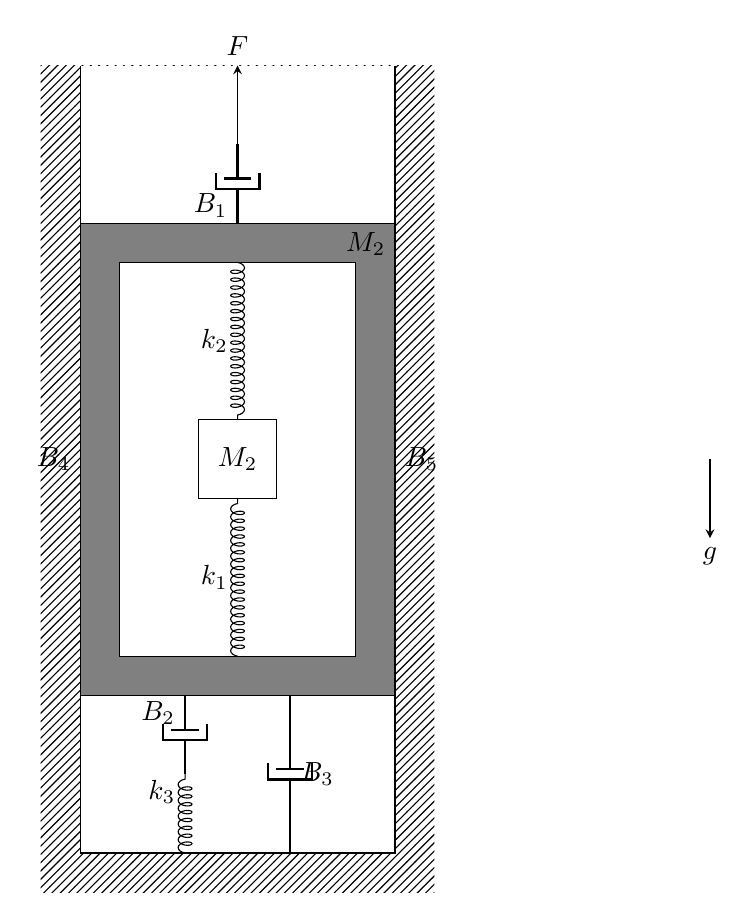
\begin{tikzpicture}
			\tikzstyle{spring}=[decorate, decoration={coil, segment length = 0.1cm}]
			\tikzstyle{damper}=
			[
				thick,
				decoration=
				{
					markings,  
					mark connection node=dmp,
					mark=at position 0.5 with 
			  		{
					    \node (dmp) [thick,inner sep=0pt,transform shape,rotate=-90,minimum width=15pt,minimum height=3pt,draw=none] {};
					    \draw [thick] ($(dmp.north east)+(2pt,0)$) -- (dmp.south east) -- (dmp.south west) -- ($(dmp.north west)+(2pt,0)$);
					    \draw [thick] ($(dmp.north)+(0,-5pt)$) -- ($(dmp.north)+(0,5pt)$);
					}
				}
				,decorate
			]
			\tikzstyle{ground}=[fill,pattern=north east lines,draw=none,minimum width=0.75cm,minimum height=0.3cm]
			\def\h{10};
			\def\l{4};
			\def\F{1};
			\def\ground{0.5};
			\def\y{2};
			\def\t{0.5};

			\begin{scope}
				\draw [ground] ($ (0,\h) + (-\ground,0) $) rectangle ($ (\l,0) + (\ground,-\ground) $);
				\draw [fill = white] (0,\h) -- (0,0) -- (\l,0) -- (\l,\h);
			\end{scope}

			\begin{scope}
				\draw [fill = gray] ($ (0,0) + (0,\y) $) rectangle ($ (\l,\h) + (0,-\y) $) node [below left] {$M_2$};
				\draw [fill = white] ($ (0,0) + (0,\y) + (\t,\t) $) rectangle ($ (\l,\h) + (0,-\y) + (-\t,-\t) $);
			\end{scope}

			\begin{scope}
				\draw [spring] (\l/3,0) -- ++(0,\y/2) node [midway, above left] {$k_3$};
				\draw [damper] ($ (\l/3,0) + (0,\y/2) $) -- ++(0,\y/2) node [midway, above left] {$B_2$};

				\draw [damper] (2*\l/3,0) -- ++(0,\y) node [midway, right] {$B_3$};
			\end{scope}

			\begin{scope}
				\draw ($ (\l/2,\h/2) + (-\t,-\t) $) rectangle ($ (\l/2,\h/2) + (\t,\t) $);
				\node at (\l/2,\h/2) {$M_2$};
				\draw [spring] ($ (0,0) + (\l/2,\y + \t) $) -- ($ (\l/2,\h/2) + (0,-\t) $) node [midway, left] {$k_1$};
				\draw [spring] ($ (0,\h) + (\l/2,-\y - \t) $) -- ($ (\l/2,\h/2) + (0,\t) $) node [midway, left] {$k_2$};
			\end{scope}

			\begin{scope}
				\draw [damper] (\l/2,\h/2 + \y + 2*\t) -- ++(0,\F) node [midway, below left] {$B_1$};
				\draw [-stealth] ($ (\l/2,\h/2 + \y + 2*\t) + (0,\F) $) -- ++(0,\F) node [above] {$F$};
			\end{scope}

			\begin{scope}
				\node [left] at (0,\h/2) {$B_4$};
				\node [right] at (\l,\h/2) {$B_5$};
			\end{scope}

			\begin{scope}
				\draw [-stealth] (2*\l,\h/2) -- ++(0,-\F) node [below] {$g$};
			\end{scope}
		\end{tikzpicture}
	\end{figure}
	The illustration describes a system of an elevator with mass $M_1$, and a mass $M_2$ connected to the elevator.
	The positive direction is defined upwards.
	It is given that $\forall i$,
	\begin{align*}
		B_i & = B \\
		k_i & = k
	\end{align*}
	\begin{enumerate}
		\item
			Draw an equivalent electrical diagram.
		\item
			Find the velocities of the masses $M_1$ and $M_2$ in the steady state.
			Assume a constant force $f(t) = f_0 \delta_{-1}(t)$.
	\end{enumerate}
\end{question}

\begin{solution}
	\begin{enumerate}
		\item
			The equivalent electrical system is
			\begin{figure}[H]
				\centering
				\begin{circuitikz}[scale = 0.8]
					\draw (0,0) to [american current source = $F$] (0,4);
					\draw (2,0) to [C = $M_1$] (2,4);
					\draw (4,4) to [american current source = $M_1 g$] (4,1) to (4,0);
					\draw (6,0) to [R = $\frac{1}{B_4}$] (6,4);
					\draw (8,0) to [R = $\frac{1}{B_5}$] (8,4);
					\draw (10,0) to [L = $\frac{1}{k_3}$] (10,2);
					\draw (10,2) to [R = $\frac{1}{B_2}$] (10,4);
					\draw (12,0) to [C = $M_2$] (12,4);
					\draw (14,0) to [R = $\frac{1}{B_3}$] (14,4);
					\draw (16,4) to [american current source = $M_2 g$] (16,0);

					\draw (0,4) to [R = $\frac{1}{B_1}$] (2,4);
					\draw (2,4) to (12,4);
					\draw (12,4) to [L = $\frac{1}{k_2}$] (14,4);
					\draw (14,4) to (16,4);

					\draw (12,4) to (12,6) to [L = $\frac{1}{k_1}$] (14,6) to (14,4);

					\draw (0,0) to (16,0);

					\draw (2,4) circle (1pt) node [above] {$v_1$};
					\draw (12,4) circle (1pt) node [above] {$v_1$};
				\end{circuitikz}
			\end{figure}
		\item
			In the steady state, all capacitors are equivalent to breaks and all inductors are equivalent to shorts.\\
			Therefore, the equivalent circuit is
			\begin{figure}[H]
				\centering
				\begin{circuitikz}[scale = 0.8]
					\draw (0,0) to [american current source = $F$] (0,4);
					\draw (2,0) to [open] (2,4);
					\draw (4,4) to [american current source = $M_1 g$] (4,1) to (4,0);
					\draw (6,0) to [R = $\frac{1}{B_4}$] (6,4);
					\draw (8,0) to [R = $\frac{1}{B_5}$] (8,4);
					\draw (10,0) to [closed] (10,2);
					\draw (10,2) to [R = $\frac{1}{B_2}$] (10,4);
					\draw (12,0) to [open] (12,4);
					\draw (14,0) to [R = $\frac{1}{B_3}$] (14,4);
					\draw (16,4) to [american current source = $M_2 g$] (16,0);

					\draw (0,4) to [R = $\frac{1}{B_1}$] (2,4);
					\draw (2,4) to (12,4);
					\draw (12,4) to [closed] (14,4);
					\draw (14,4) to (16,4);

					\draw (12,4) to (12,6) to [closed] (14,6) to (14,4);

					\draw (0,0) to (16,0);

					\draw (2,4) circle (1pt) node [above] {$v_1$};
					\draw (12,4) circle (1pt) node [above] {$v_1$};
				\end{circuitikz}
			\end{figure}
			Therefore, substituting the given values for all $B_i$ and $k_i$, the equivalent circuit is
			\begin{figure}[H]
				\centering
				\begin{circuitikz}[scale = 0.8]
					\draw (0,0) to [american current source = $F$] (0,4);
					\draw (2,0) to [open] (2,4);
					\draw (4,4) to [american current source = $M_1 g$] (4,1) to (4,0);
					\draw (6,0) to [R = $\frac{1}{B}$] (6,4);
					\draw (8,0) to [R = $\frac{1}{B}$] (8,4);
					\draw (10,0) to [closed] (10,2);
					\draw (10,2) to [R = $\frac{1}{B}$] (10,4);
					\draw (12,0) to [open] (12,4);
					\draw (14,0) to [R = $\frac{1}{B}$] (14,4);
					\draw (16,4) to [american current source = $M_2 g$] (16,0);

					\draw (0,4) to [R = $\frac{1}{B}$] (2,4);
					\draw (2,4) to (12,4);
					\draw (12,4) to [closed] (14,4);
					\draw (14,4) to (16,4);

					\draw (12,4) to (12,6) to [closed] (14,6) to (14,4);

					\draw (0,0) to (16,0);

					\draw (2,4) circle (1pt) node [above] {$v_1$};
					\draw (12,4) circle (1pt) node [above] {$v_1$};
				\end{circuitikz}
			\end{figure}
			Therefore, simplifying, the circuit is equivalent to
			\begin{figure}[H]
				\centering
				\begin{circuitikz}[scale = 1.5]
					\draw (0,0) to [american current source = $F$] (0,4);
					\draw (2,4) to [american current source = $(M_1 + M_2) g$] (2,1) to (2,0);
					\draw (4,0) to [R = $\frac{1}{4 B}$] (4,3) to (4,4);

					\draw (0,4) to [R = $\frac{1}{B}$] (2,4);
					\draw (2,4) to (4,4);

					\draw (0,0) to (4,0);

					\filldraw (4,4) circle (1pt) node [above] {$v_1 = v_2$};
				\end{circuitikz}
			\end{figure}
			Therefore, the velocities of the masses are equal, and are
			\begin{equation*}
				v_1 = v_2 = \left( F - (M_1 + M_2) g \right) \frac{1}{4 B}
			\end{equation*}
	\end{enumerate}
\end{solution}

\end{document}
